\documentclass[12pt]{article}

\usepackage{graphicx}
\usepackage{amsmath}
\usepackage{amssymb}
\usepackage{natbib}
\usepackage{amsfonts}
\usepackage{multicol}
\usepackage{float}
\usepackage{oldgerm}
\usepackage{bm}
\usepackage{mathtools}
\usepackage{wrapfig}
\usepackage{fancyhdr}
\usepackage[export]{adjustbox}
\usepackage{xcolor}

\pagestyle{empty}

\newcommand{\Avec}{\mathbf A}
\newcommand{\Bvec}{\mathbf B}
\newcommand{\Dvec}{\mathbf D}
\newcommand{\Evec}{\mathbf E}
\newcommand{\Fvec}{\mathbf F}
\newcommand{\Jvec}{\mathbf J}
\newcommand{\Lvec}{\mathbf L}
\newcommand{\Mvec}{\mathbf M}
\newcommand{\Pvec}{\mathbf P}
\newcommand{\Svec}{\mathbf S}
\newcommand{\avec}{\mathbf a}
\newcommand{\bvec}{\mathbf b}
\newcommand{\dvec}{\mathbf d}
\newcommand{\evec}{\mathbf e}
\newcommand{\fvec}{\mathbf f}
\newcommand{\jvec}{\mathbf j}
\newcommand{\kvec}{\mathbf k}
\newcommand{\nvec}{\mathbf n}
\newcommand{\pvec}{\mathbf p}
\newcommand{\rvec}{\mathbf r}
\newcommand{\svec}{\mathbf s}
\newcommand{\vvec}{\mathbf v}
\newcommand{\xvec}{\mathbf x}
\newcommand{\yvec}{\mathbf y}
\newcommand{\zvec}{\mathbf z}
\newcommand{\nablav}{\boldsymbol{\nabla}}
\newcommand{\nablavector}{\vec \nabla}
\newcommand{\alphavec}{\boldsymbol{\alpha}}
\newcommand{\phivec}{\boldsymbol{\phi}}
\newcommand{\thetavec}{\boldsymbol{\theta}}
\newcommand{\omegavec}{\boldsymbol{\omega}}
\newcommand{\tauvec}{\boldsymbol{\tau}}
\newcommand{\ezero}{\varepsilon_{0}}
\newcommand{\mzero}{\mu_{0}}
\newcommand{\mubold}{\boldsymbol{\mu}}
\newcommand{\uniti}{\hat{\boldsymbol{\imath}}}
\newcommand{\unitj}{\hat{\boldsymbol{\jmath}}}
\newcommand{\unitk}{\hat{\boldsymbol{\mathit{k}}}}
\newcommand{\unitn}{\hat{\mathbf n}}
\newcommand{\unitr}{\hat{\mathbf r}}
\newcommand{\unitphi}{\hat{\boldsymbol{\phi}}}
\newcommand{\unittheta}{\hat{\boldsymbol{\theta}}}

\newcommand{\bit}{\begin{itemize}}
\newcommand{\eit}{\end{itemize}}

\setlength{\headsep}{0.5cm}
\setlength{\oddsidemargin}{-0.5cm}
\setlength{\textwidth}{16.5cm}
\setlength{\textheight}{24cm}
\voffset = -2cm

\pagestyle{fancy}
\fancyhf{}
\rfoot{
\includegraphics[width=1.0in]{cnm.png}}
\lfoot{ENGR 2910 Homework 7}

\begin{document}

%{\bf \underline{STUDENT NAME}:} 
%\vspace{1cm}

\begin{center}
\hfil
%\begin{wrapfigure}{l}{0.5in} 
%    
\includegraphics[width=0.5in]{cnm.png}
%\end{wrapfigure}
{\large\bf {ENGR 2910-101: Circuit Analysis}}
\hfill Instructor: Leo Silbert \\
Homework 7: 10/20/21 \hfill Due: 10/27/21\\
\hrulefill\\
\end{center}

%{\em Show all your working to ensure you obtain full points. Partial
%  credit will be given for correct algebraic steps if you fail to
%  obtain the correct final answer.}\\

%\newpage


\noindent
{\bf Question 1} [10]

Use the node-voltage method to find: $v_{o}$ and the power developed in the voltage source.

\begin{figure}[h!]
  \centering 
 \vspace{-0.1in}
 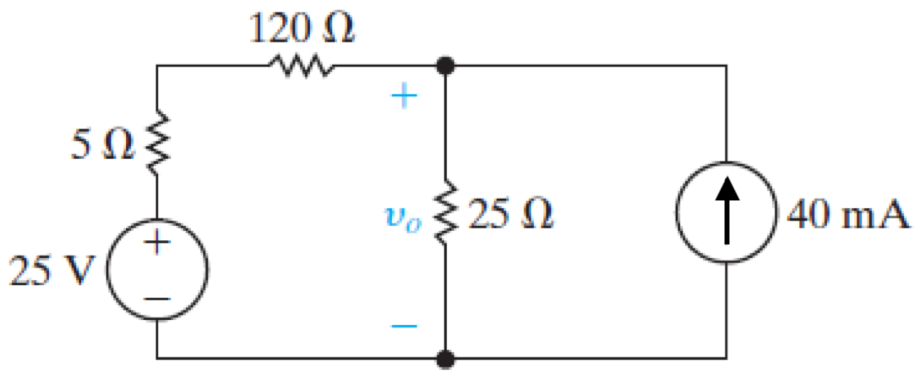
\includegraphics[clip,width=0.6\textwidth]{Fig4-6-v2.png}
 %\vspace{-0.1in}
\end{figure}
%For the circuit shown above,
%\bit 
%
%\item[(i)] 

%\item[(ii)]
%
%calculate the power developed by the current and the voltage sources,
% 
%\item[(iii)]
%
%the power dissipated in each of the three resistors. 
%
%\eit

\vspace{0.1in}
\noindent
{\bf Question 2} [10]

Use the node-voltage method to find $v_{1}$ and $v_{2}$ in the circuit below.
\begin{figure}[h!]
     \centering
\vspace{-0.1in}
     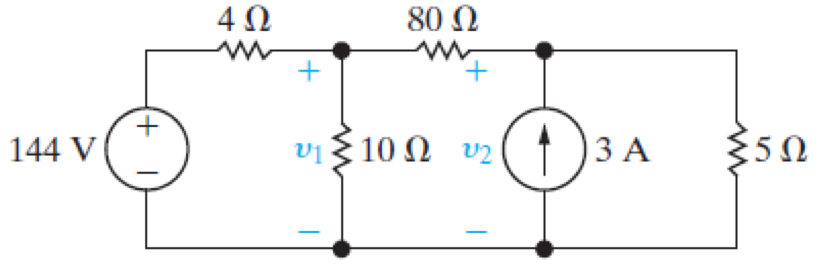
\includegraphics[clip,width=0.7\textwidth]{Fig4-11.png}
\vspace{-0.15in}
\end{figure}


\noindent
{\bf Question 3} [10]

Use the node-voltage method to find the voltages shown, $v_{1}$, $v_{2}$, and $v_{3}$.
\begin{figure}[h!]
  \centering 
  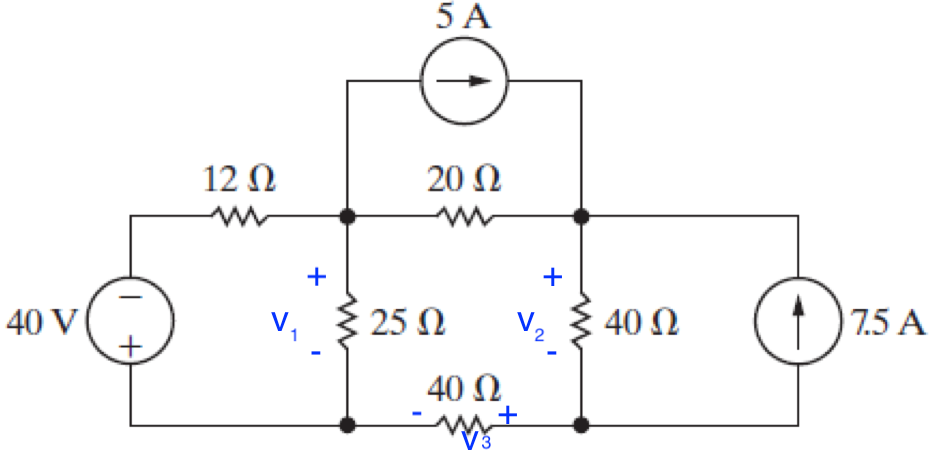
\includegraphics[clip,width=0.7\textwidth]{Fig4-15.png}
\end{figure}

\newpage
\noindent
{\bf Question 4} [10]

Use the node-voltage method to find $v_{o}$ in the circuit shown below.

\vspace{0.1in}
\begin{figure}[h]
  \centering 
  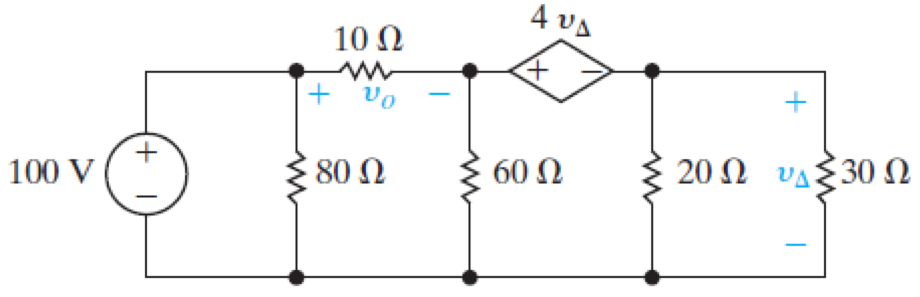
\includegraphics[clip,width=0.8\textwidth]{Fig4-28.png}
\end{figure}

\vspace{0.1in}
\noindent
{\bf Question 5} [10]

Use the node-voltage method to find: [Hints: identify the supernode and also use the node labeled {\color{red} a}.]
\begin{figure}[h!]
\centering 
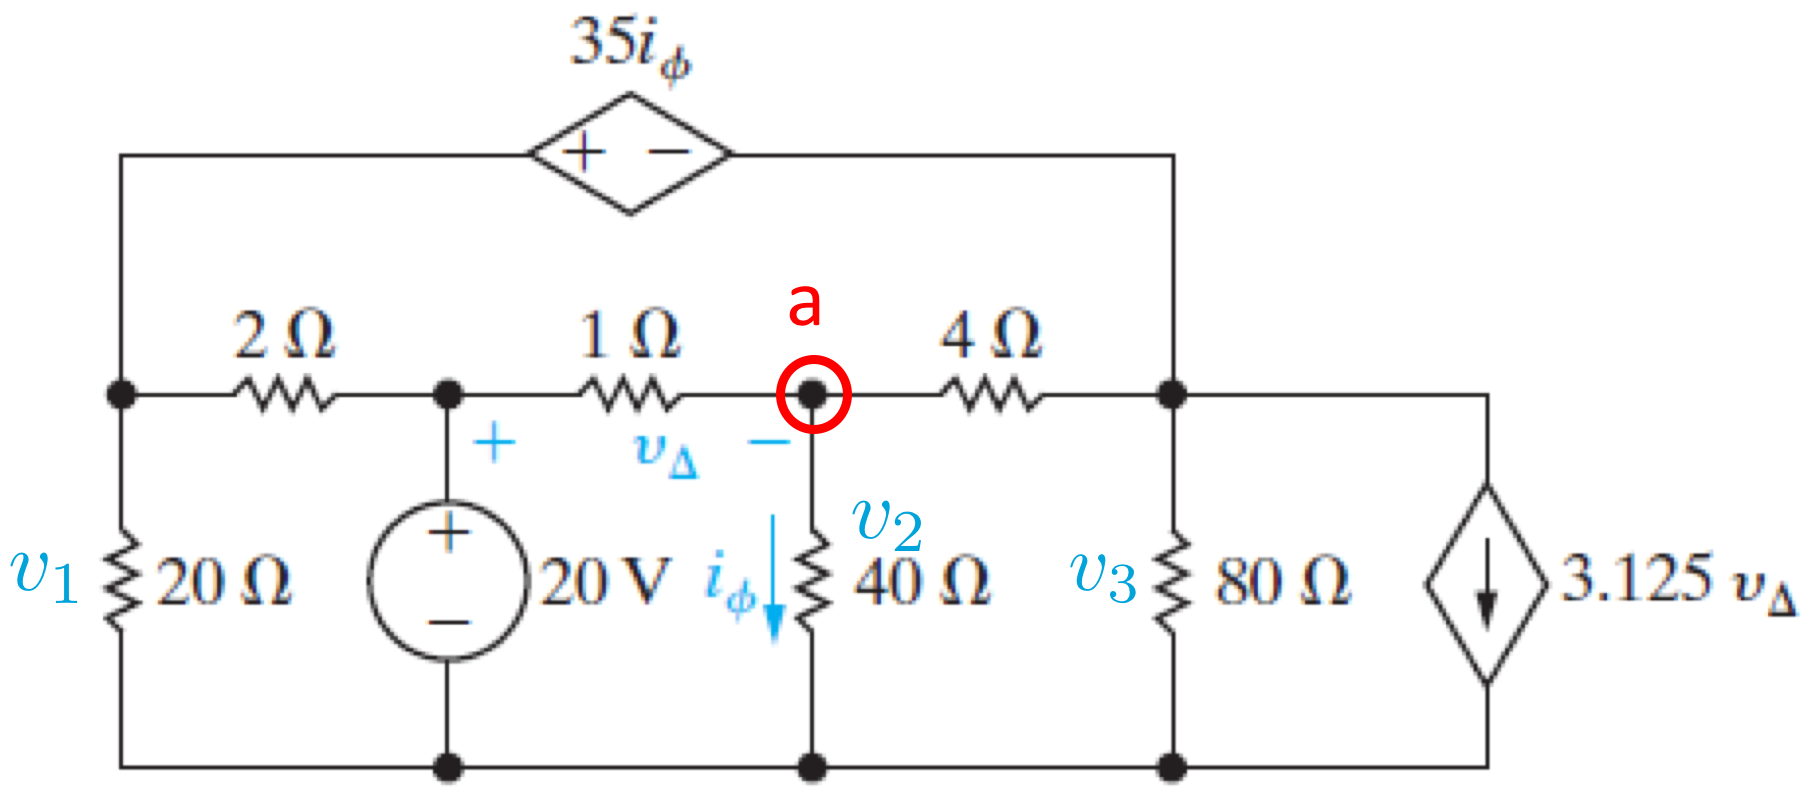
\includegraphics[clip,width=0.8\textwidth]{Fig4-29.png}
\end{figure}

\begin{enumerate}[(a)]
\item
\end{enumerate}

\item[(i)]

the voltage across the 20 $\Omega$ resistor, $v_{1}$, 

\item[(ii)]

the voltage across the 40 $\Omega$ resistor, $v_{2}$, 

\item[(iii)]

the voltage across the 80 $\Omega$ resistor, $v_{3}$, 

\item[(iv)]

the controlling voltage, $v_{\Delta}$, 

\item[(v)]

the controlling current, $i_{\phi}$. 

\eit

\end{document}
